\documentclass[../../index.tex]{subfiles}

\begin{document}
\chapter{Measuring the Strong Coupling}


\begin{wraptable}{l}{7cm}
  \vspace{-1cm} \small
  \caption{Timeline}
  \begin{tabular}{@{\,}r <{\hskip 5pt} !{\foo}
      >{\raggedright\arraybackslash}p{5cm}}
    \toprule
    \addlinespace[1.5ex]
    1991 & \cite{Braaten1991}: Systematic description, including \textsc{np} corrections to extract \(\alpha_s\) from \(R_\tau\). \\
    1992 & \cite{LeDiberder1992}: Introducing weights and fit methodology. \\
    1993 & \cite{Aleph1993} \textsc{aleph} measures the strong coupling constant \(\alpha_s\).\\
    1998 & \cite{Opal1998} \textsc{opal} measures the strong coupling constant \(\alpha_s\).\\
    2005 & \cite{Aleph2005} \textsc{aleph} improves their data. \\
    2011 & \cite{Boito2011a,Boito2010}: Include \textsc{dv}. Discover inconsistencies in \textsc{aleph} data. \\
    2014 & \cite{Davier2013} \textsc{aleph} updates their data. \\
  \end{tabular}
  \label{table:AlphasTauTimeline}
\end{wraptable}
The strong coupling has been measured for many years from hadronic \(\tau\)
decays. An overview of the recently, but different, \(\alpha_s\) values can be
seen in \cref{fig:historicAlphasComparison}.
\begin{figure}
  \centering
  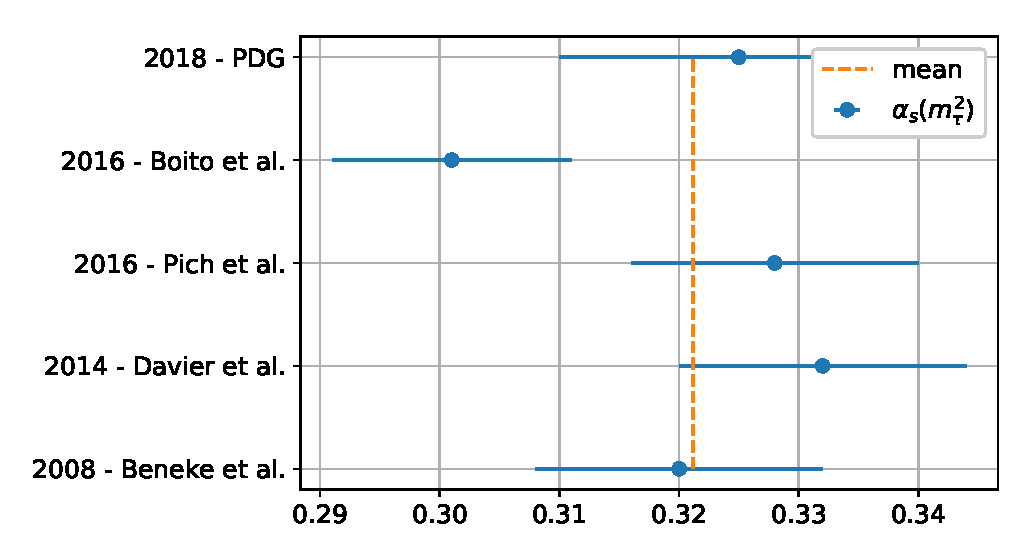
\includegraphics[width=\textwidth]{./images/historicAlphasComparison.eps}
  \caption{Recent values for \(\alpha_s(m_\tau^2)\) from hadronic \(\tau\)
    decays. The dashed line represents the mean value of \(0.3212\). The values
    are taken from \cite{PDG2018, Boito2016, Pich2016, Davier2013, Beneke2008},
    from top to bottom.}
  \label{fig:historicAlphasComparison}
\end{figure}
Until today most of the applied \textsc{qcdsr} to \(\tau\) decays are based on
the methodology developed in the early nineties by Braaten, Pich and Narison
\cite{Braaten1991}. They gathered at this time available perturbative and
\textsc{np} contributions to extract the strong coupling from comparing their
theoretical results to the known inclusive hadronic \(\tau\) decay ratio
\(R_\tau\). Pich together with Le Diberder then formulated the fitting strategy
of applying multiple moments of different weights to extract \(\alpha_s\)
parallel to Wilson coefficients of the \textsc{ope} \cite{LeDiberder1992}, which
later has been applied as standard in the \textsc{aleph} \cite{Aleph1993} as
well as the \textsc{opal} \cite{Opal1998} detectors. For the next ten years, the
methodology of extracting the strong coupling did not experience any major
changes until 2011 when Boito, Cata, Golterman, Jamin, Osborn and Peris
\cite{Boito2011a} applied a duality model to include known \textsc{dv} effects
to the \textsc{qcd} analysis of \(\tau\) decays. The groups around Boito and
Pich have different opinions on the importance of the newly introduced duality
model \cite{Pich2016,Boito2016,} and consequently, we want to deliver a third,
opinion on the subject, favouring fits without the duality model.


\section{Fit Strategy}
The objective of this work is to extract \(\alpha_s\) and argue about the
importance of \textsc{dv}. Apart from the two main objectives, we want to
analyse the contribution of higher order \textsc{ope} contributions up to
dimension ten.

For performing the fits we had to restrict ourselves to the following
approximations
\begin{itemize}
\item We used the \textsc{pt} expansion of the Adler function up to fifth order,
  including the educated guess of \(c_{5,1}\).
\item We ignore the dimension two \textsc{ope} contributions as they are
  proportional to the quark masses and we work in the chiral limit.
\item We neglect the logarithmic contributions to the dimension four
  \textsc{ope} contributions.
\item For the higher dimensions of the \textsc{ope} \(D=6,8,\dots\) we
  parametrise their contributions as a constant divided by the corresponding
  power in \(s\)
  \begin{equation}
    \left D_{V/A}^{(1+0)}\right\vert_{D=d} \equiv \frac{\rho^{(d)}}{s^{d/2}}.
  \end{equation}
\end{itemize}

Our fitting strategy will be in choosing weights of a lower and higher pinching.
Lower pinched weights should be affected by \textsc{dv}, while higher pinched
weights should be protected from \textsc{dv}. As a result in comparing different
fits of lower and higher pinched weights, it should be possible to argue about
the strength of the \textsc{dv} that are (or are not) present.

Our hypothesis is that \textsc{dv} are small enough for fits of the combined
vector and axial\-/vector channel in combination with pinched weights.
Consequently, we can extract parameters, like the strong coupling \(\alpha_s\)
from \(\tau\) decays to high precision without a \textsc{dv} model.

We will perform our analysis of the \textsc{dv} in the framework of
\textsc{fopt} for weights without a monomial term \(x\). For weights including a
monomial term \(x\), we will apply the \textsc{bs}. To define a fit we have to
choose a weight \(\omega\) and a momentum \(s_0\). The only restriction from
choosing a weight is, that, it has to be analytic, leaving us with a variety of
choices. For our strategy, we have chosen three categories of weights, each of
them containing fits with three or four different \(\omega\). A table with an
overview of all used weights is given in \cref{table:fitCategories}.
\begin{table}
  \centering
  \begin{tabular}{ccccc}
    \toprule
    & Symbol & Term & Expansion & \textsc{ope} Contributions \\
    \midrule
    \parbox[t]{2mm}{\multirow{3}{*}{\rotatebox[origin=c]{90}{\small Pinched}}} & \(\omega_\tau\) & \((1-x)^2(1+2x)\) & \(1 - 3x^2 + 2x^3\) & \(D6, D8\) \\
    & \(\omega_{cube}\) & \((1-x)^3(1+3x)\) & \(1 - 6x^2 + 8x^3 - 3x^4\) & \(D6, D8, D10\) \\
    & \(\omega_{quartic}\) & \((1-x)^4(1+3x)\) & \(1 - 10x^2 + 20x^3 - 15x^4 + 4x^5\) & \(D6, D8, D10, D12\) \\
    \midrule
    \parbox[t]{2mm}{\multirow{3}{*}{\rotatebox[origin=c]{90}{\small Monomial}}} & \(\omega_{M2}\) & \(1 - x^2\) & \(1-x^2\) & \(D6\) \\
    & \(\omega_{M3}\) & \(1 - x^3\) & \(1 - x^3\) & \(D8\) \\
    & \(\omega_{M4}\) & \(1 - x^4\) & \(1 - x^4\) & \(D10\) \\
    \midrule
    \parbox[t]{2mm}{\multirow{4}{*}{\rotatebox[origin=c]{90}{\small Pinched \(+ x\)}}} & \(\omega_{1,0}\) & \((1 - x)\) & \(1 - x\) & \(D4\) \\
    & \(\omega_{2,0}\) & \((1 - x)^2\) & \(1 - 2x + x^2\) & \(D4, D6\) \\
    & \(\omega_{3,0}\) & \((1 - x)^3\) & \(1 - 3x + 3x^2 - x^3\) & \(D4, D6, D8\) \\
    & \(\omega_{4,0}\) & \((1 - x)^4\) & \(1 - 4x + 6x^2 - 4x^3 + x^4\) & \(D4, D6, D8, D10\) \\
    \bototmline
  \end{tabular}
  \caption{Displaying three categories of fits, each containing three weights
    with their corresponding mathematical expression and the \textsc{ope}
    contributions the fitted integral momentum will be sensitive to.}
  \label{table:fitCategories}
\end{table}
To test the stability of the fitted values and have enough \textsc{dof} to fit
the higher \textsc{ope} contributions we furthermore fit every weight for
various momenta \(s_0\).

To probe the validity of \textsc{fopt} we apply the \textsc{bs} for weights
without a monomial term \(x\). If \textsc{fopt} is valid the parameters obtained
from both approaches, the Borel model and \textsc{fopt}, should be similar.
As \textsc{cipt} in general yields different results for the strong coupling and
higher order contributions as \textsc{fopt}, it should be the worse framework if
\textsc{bs} and \textsc{fopt} lead to similar parameter values.


\section{Fits}
In the following, we will show the results of each of the three previously
mentioned fit categories.

The first category contains the \textit{pinched weights without a monomial term
  x}. The chosen weights are double (\(\omega_\tau\)), triple
(\(\omega_{cube}\)) and quadruple (\(\omega_{quartic}\)) pinched and do not
contain a monomial term \(x\). An \(x\) term would make the fits sensitive to
the \(D=4\) \textsc{ope} contribution, which causes an unreliable perturbative
expansion \cite{Beneke2012}. The higher the pinching, the higher the suppression
of \textsc{dv}. Consequently, if we obtain stable values for \(\alpha_s\) from
the different pinched fits we should expect the \textsc{dv} to have no influence
on the value of the strong coupling. The different weights imply an increasing
number of active \textsc{ope} contributions \(D_6, D_8, D_{10}\) and \(D_{12}\),
which can be used to probe the stability of higher order \textsc{ope}
contributions and to test for the convergence of the \textsc{ope}.

The second category contains the \textit{single pinched monomial weights}. In
this case, all of the weights are only single pinched and, as in the first
category, do not carry a monomial term \(x\). Consequently, if \textsc{dv}
affect the fits we should notice different fitting results in comparison to the
fits of the first category. Furthermore, the single pinched moments only carry
two parameters, the strong coupling and an \textsc{ope} Wilson coefficient. Thus
we can further compare the \(\rho^{(6)}, \rho^{(8)}\) and \(\rho^{(10)}\) Wilson
coefficients and argue about the stability of the fits.

The third and last category contains a similar pinching as the first category,
but this time contains a monomial term in \(x\). Consequently, these fits are
unreliable in the framework of \textsc{fopt} and we have to apply the
\textsc{bs}. Following the logic of the second and first category, we then can
compare the result to analyse the role of \textsc{dv} and compare the
\textsc{ope} contributions.

\subsection{Pinched Weights without a Monomial term \(x\)}

\subsubsection{Kinematic Weight: \(\omega_{\tau}(x) \equiv (1-x)^2(1+2x)\)}
We previously encountered the kinematic weight in \cref{eq:kinematicWeight}. It
is a polynomial weight function, defined as \(\omega_\tau(x) = (1-x)^2(1+2x)\),
double pinched, contains the unity and does not contain a term proportional to
\(x\). Consequently, it is an optimal weight \cite{Beneke2012}. As a doubled
pinched weight it should have good suppression of \textsc{dv} contributions and
its polynomial contains terms proportional to \(x^2\) and \(x^3\), which makes
it sensitive to the dimension six and eight \textsc{ope} contributions. The fits
have been performed within the framework of \textsc{fopt} for different numbers
of \(s_0\). The momentum sets are characterised by its lowest energy
\(s_{min}\). We fitted values down to \SI{1.5}{\giga\eV}. Going to lower
energies is questionable due to the coupling constant becoming large, which
implies a breakdown of \textsc{pt}. Furthermore, it bears the risk to be
affected by the \(\rho(770)\) and \(a_1\) peaks in the vector and axial\-/vector
spectral function, which we cannot model within the framework of the
\textsc{ope}. For the three fitting parameters \(\alpha_s, \rho^{(6)}\) and
\(\rho^{(8)}\) we have given the results in \cref{table:fitWKinAlD6D8} and
graphically in \cref{fig:fitWKinAlD6D8}.
\begin{table}
  \centering
  \begin{tabularx}{\textwidth}{cccYYYY}
    \toprule
    & \(s_{min}\) & \#\(s_0\)s & \(\alpha_s(m_\tau^2)\) & \(\rho^{(6)}\) & \(\rho^{(8)}\) & \(\chi^2/dof\)  \\
    \midrule
    \parbox[t]{2mm}{\multirow{1}{*}{\rotatebox[origin=c]{90}{\textsc{bs}}}}
    & 2.200 & 7 & 0.3274(42) & -0.82(21) & -1.08(40) & 0.21 \\
    \midrule
    \parbox[t]{2mm}{\multirow{5}{*}{\rotatebox[origin=c]{90}{\textsc{fopt}}}}
    % 1.500 & 23 & 0.3255(13) & -0.441(10) & -0.2909(34) & 2.00 \\
    % 1.525 & 22 & 0.3255(18) & -0.440(36) & -0.288(45) & 2.10 \\
    % 1.550 & 21 & 0.3265(16) & -0.478(36) & -0.343(50) & 1.81 \\
    % 1.575 & 20 & 0.3269(22) & -0.493(47) & -0.365(58) & 1.86 \\
    % 1.600 & 19 & 0.3272(23) & -0.506(51) & -0.384(64) & 1.94 \\
    % 1.625 & 18 & 0.3284(24) & -0.540(53) & -0.433(68) & 1.788 \\
    % 1.650 & 17 & 0.3283(24) & -0.550(57) & -0.448(74) & 1.90 \\
    % 1.675 & 16 & 0.3284(24) & -0.549(57) & -0.448(79) & 2.04 \\
    % 1.700 & 15 & 0.3281(24) & -0.538(63) & -0.430(87) & 2.19 \\
    % 1.750 & 14 & 0.3291(26) & -0.581(71) & -0.50(10) & 2.21 \\
    % 1.800 & 13 & 0.3293(27) & -0.589(77) & -0.51(11) & 2.43 \\
    % 1.850 & 12 & 0.3281(28) & -0.537(85) & -0.42(13) & 2.5 \\
    % 1.900 & 11 & 0.3272(29) & -0.493(93) & -0.35(15) & 2.65 \\
    % 1.950 & 10 & 0.3232(32) & -0.31(11) & -0.01(18) & 1.13 \\
    % 2.000 & 9 & 0.3234(34) & -0.32(12) & -0.03(21) & 1.31 \\
    & 2.100 & 8 & 0.3256(38) & -0.43(15) & -0.25(28) & 1.30 \\
    & \cellcolor{primary}2.200 & \cellcolor{primary}7 & \cellcolor{primary}0.3308(44) & \cellcolor{primary}-0.72(20) & \cellcolor{primary}-0.85(38) & \cellcolor{primary}0.19 \\
    & 2.300 & 6 & 0.3304(52) & -0.69(25) & -0.80(50) & 0.25 \\
    & 2.400 & 5 & 0.3339(70) & -0.91(39) & -1.29(83) & 0.10 \\
    & 2.600 & 4 & 0.3398(15) & -1.3(1.0) & -2.3(2.5) & 0.01  \\
    \bottomrule
  \end{tabularx}
  \caption{Table of our fitting values of \(\alpha_s(m_\tau^2), \rho^{(6)}\) and
    \(\rho^{(8)}\) for the kinematic weight \(\omega(x)=(1-x)^2(1+2x)\) using
    \textsc{fopt} ordered by increasing \(s_{min}\). The errors are given in
    parenthesis after the observed value.}
  \label{table:fitWKinAlD6D8}
\end{table}
\begin{figure}
  \centering \includegraphics[width=\textwidth]{./images/fitWKinAlD6D8.eps}
  \caption{Fitting values of \(\alpha_s(m_\tau^2), \rho^{(6)}\) and
    \(\rho^{(8)}\) for the kinematic weight \(\omega(x)=(1-x)^2(1+2x)\) using
    \textsc{fopt} for different \(s_{min}\). The left graph plots
    \(\alpha_s(m_\tau^2)\) for different numbers of used \(s_0\)s. The right
    plot contains dimension six and eight contributions to the \textsc{ope}.
    Both plots have in grey the \(\chi^2\) per \textsc{dof}.}
  \label{fig:fitWKinAlD6D8}
\end{figure}

We only display the fits for \(s_{min}\) larger than \SI{2.1}{\giga\eV}. We
noted a jump between the \(s_{min}=\SI{2.1}{\giga\eV}\) and
\(s_{min}=\SI{2.2}{\giga\eV}\) of the \(\chi^2/dof\) from \(0.19\) to \(1.3\).
We consequently discarded fits with a \(s_{min}<\SI{2.2}{\giga\eV}\), as fits
lower \(s_{min}\) behave more stable\footnote{As will be seen by comparing the
  kinematic weight with the cubic and quartic weight}. The values with fewer
momenta are preferred by us due to two reasons. First, below energies of
\SI{2.2}{\giga\eV}, we have to face the problematic influence of increasing
resonances. Second, we will see, that the values obtained from the lower moment
fits are more compatible with our other fits series. We further discarded the
fit with four \(s_0\)s momenta, which has very small \(\chi^2/dof=0.01\). This
is due to the fact, that we have four \(s_0\)s momenta to fit three parameters,
which leaves us with too few \textsc{dof}.

The selected fits with \(8\-/10\) momenta have a small \(\chi^2\) per
\textsc{dof}. The fitted parameters, \(\alpha_s, \rho^{(6)}\) and \(\rho^{(8)}\)
are in good agreement with each other. For all fits, we have a good convergence
of the \textsc{ope}. For later comparisons, we will focus on the fit right below
the \(\chi^2/dof\) threshold. For the kinematic weight we get for the strong
coupling, \(D=6\) and \(D=8\) contributions:
\begin{equation}
  \label{eq:wKinResult}
  \alpha_s(m_\tau^2) = 0.3308(44), \quad \rho^{(6)} = -0.72(20) \quad \text{and} \quad
  \rho^{(8)} = -0.85(38).
\end{equation}

We further tested the stability of dimension six and eight contributions to the
\textsc{ope} within the same fit series but for a fixed value of the strong
coupling \(\alpha_s(m_\tau^2)=0.3179\). The values for \(\rho^{(6)}\) and
\(\rho^{(8)}\) are larger than the values given in our final results from
\cref{table:fitWKinAlD6D8}. This is explained with a smaller contribution from
the strong coupling, which has to be compensated by larger \textsc{ope}
contributions.

Additionally, we applied the \textsc{bs} for the fit below the \(\chi^2\)
threshold containing seven \(s_0\)s. Even though we used a different framework
than \textsc{fopt} the results are compatible. This further underlines the good
results of the kinematic weight fit and can be seen as an indicator for
\textsc{fopt} being the superior framework as compared to \textsc{cipt}, which
already has been argued in \cite{Beneke2008}.


\subsubsection{Cubic Weight: \(\omega_{cube}(x) \equiv (1-x)^3(1+3x)\)}
\label{sec:cubicWeight}
To further consolidate the results from the kinematic weight, we tested a weight
of higher pinching, which should suppress \textsc{dv} more than a double pinched
weight. Consequently, if we obtain similar results to our previous fits we could
exclude \textsc{dv} effects for the kinematic weight. On the other hand, any
differences to the previous fit would indicate present \textsc{dv} in the
kinematic weight. Our \textit{cubic} weight will be triple pinched and optimal,
as it does not contain a monomial term \(x\). It is due to its polynomial
structure sensitive to the dimensions six, eight and ten contributions of the
\textsc{ope}, which yields one more parameter to fit than with the kinematic
weight \(\omega_\tau\). The fitting results can be seen in
\cref{table:fitWCubicAlD6D8D10} and graphically in \cref{fig:fitWCubeAlpha}.
\begin{table}
  \centering
  \begin{tabularx}{\textwidth}{ccYYYYY}
    \toprule
    \(s_{min}\) & \#\(s_0\)s & \(\alpha_s(m_\tau^2)\) & \(\rho^{(6)}\) & \(\rho^{(8)}\) & \(\rho^{(10)}\) & \(\chi^2/dof\)  \\
    \midrule
    % 1.800 & 13 & 0.3305(37) & -0.493(76) & -0.48(12) & -0.66(20) & 2.99 \\
    % 1.850 & 12 & 0.3303(37) & -0.482(68) & -0.456(100) & -0.62(17) & 3.35 \\
    % 1.900 & 11 & 0.3249(29) & -0.280(20) & -0.088(21) & 0.088(55) & 1.58 \\
    % 1.950 & 10 & 0.3237(26) & -0.232(25) & 0.005(42) & 0.275(93) & 1.67 \\
    2.000 & 9 & 0.3228(26) & -0.196(27) & 0.075(28) & 0.420(56) & 1.96 \\
    \rowcolor{primary}
    2.100 & 8 & 0.3302(40) & -0.52(11) & -0.58(22) & -1.00(45) & 0.43 \\
    2.200 & 7 & 0.3312(43) & -0.56(12) & -0.68(23) & -1.23(50) & 0.55 \\
    2.300 & 6 & 0.336(11) & -0.78(47) & -1.17(98) & -2.38(22) & 0.29 \\
    2.400 & 5 & 0.3330(96) & -0.63(47) & -0.82(10) & -1.51(26) & 0.48 \\
    \bottomrule
  \end{tabularx}
  \caption{Table of our fitting values of \(\alpha_s(m_\tau^2), \rho^{(6)},
    \rho^{(8)}\) and \(\rho^{(10)}\) for the cubic weight
    \(\omega(x)=(1-x)^3(1+3x)\) using \textsc{fopt} ordered by increasing
    \(s_{min}\). The errors are given in parenthesis after the observed value.}
  \label{table:fitWCubicAlD6D8D10}
\end{table}
\begin{figure}
  \centering \includegraphics[width=\textwidth]{./images/fitWCubeAlD6D8D10.eps}
  \caption{Graphic representation of the fitting values of
    \(\alpha_s(m_\tau^2)\) in the left and \(\rho^{(6)}, \rho^{(8)}\) and
    \(\rho^{(10)}\) in the right plot for the cubic weight
    \(\omega(x)=(1-x)^3(1+3x)\). The fits have been performed in the
    \textsc{fopt} scheme and the data points are given with error bars and are
    ordered by increasing \(s_{min}\). The grey line displays the \(\chi^2\)
    function.}
  \label{fig:fitWCubeAlpha}
\end{figure}

We performed fits for \(s_0 \leq \SI{1.5}{\giga\eV}\), but could only reach
convergence for fits with energies larger or equal than \SI{1.8}{\giga\eV}. As
before the \(\chi^2\) makes a jump at \(s_0=\SI{2.1}{\giga\eV}\) to values per
\textsc{dof} of almost \(2\). Consequently, we excluded theses fits and focused
on fits from five to eight \(s_0\)s momenta.

The selected fits have a good \(\chi^2/dof\) and the fitted parameters,
\(\alpha_s, \rho^{(6)}, \rho^{(8)}\) and \(\rho^{(10)}\) are in agreement with
each other, except for the fit with six momenta. The fit with a
\(s_{min}=\SI{2.3}{\giga\eV}\) has the lowest \(\chi^2=0.29\) and error on
\(\alpha_s\), but takes slightly different values for the \textsc{ope} Wilson
coefficients in comparison to the other selected fits. The fit right below the
\(\chi^2/dof\) threshold for the strong coupling, \(D=6\) and \(D=8\)
contributions yields
\begin{equation}
  \begin{split}
    \alpha_s(m_\tau^2)=0.3302(40), \quad \rho^{(6)}=-0.52(11), \quad \rho^{(8)}=-0.58(22)\\
    \quad \text{and} \quad \rho^{(10)}=-1.00(45).
  \end{split}
\end{equation}
We furthermore found that the \textsc{ope} is converging, but not as fast as for
the kinematic weight. The value of \(\abs{\delta^{(8)}}\) is only half as large
as \(\abs{\delta^{(6)}}\). The values of the lower momentum count are in high
agreement with the ones obtained from the kinematic weight. The conclusions we
take from the \textit{cubic weight} are, that the kinematic weight, with its
double pinching, should sufficiently suppress any contributions from
\textsc{DV}s. If \textsc{DV} would have an effect on the kinematic weight, we
should have seen an improvement of the fits with the \textit{cubic} weight, due
to its triple pinching, which is not the case.

\subsubsection{Quartic Weight: \(\omega(x) \equiv (1-x)^4(1+4x)\)}
\label{sec:quarticWeight}
The last fits of the pinched weights without a monomial term in \(x\) uses the
\textit{quartic weight} defined as \(\omega(x) \equiv (1-x)^4(1+4x)\). It
contains five fitting parameters (\(\alpha_s, \rho^{(6)}, \rho^{(8)},
\rho^{(10)}, \rho^{(12)}\)) and did only converge for
\(s_{min}=\SI{2}{\giga\eV}\) (nine \(s_0\)s momenta). The results for the
quartic weight with a \(\chi^2\) per \textsc{dof} of \(0.67\) are given by:
\begin{equation}
  \begin{split}
    \alpha_s(m_\tau^2) &= 0.3290(11), \quad \rho^{(6)}=-0.3030(46), \quad \rho^{(8)}=-0.1874(28), \\
    \rho^{(10)} &= 0.3678(45) \quad \text{and} \quad \rho_{(12)}=-0.4071(77).
  \end{split}
\end{equation}
Due to the problematic of the fitting routing, which is caused by too many
\textsc{ope} contributions fitted simultaneously, we will discard the fitting
results for the quartic weight.


\subsection{Single Pinched Monomial Weights}
To further argue in favour of our hypothesis we want to probe some weights with
a single pinching. If \textsc{dv} play a role then we should note deviating
results to fits with higher pinchings. The advantage of these weights is that
they only let one \textsc{ope} dimension contribute, thus leaving us with only
two parameters per fit.

\subsubsection{Second Power Monomial: \(\omega_{M2}(x) \equiv 1-x^2\)}
The first weight is defined as \(\omega_{M2}(x) \equiv 1-x^2\). We only have to
fit two parameters, the strong coupling \(\alpha_s\) and the dimension six
\textsc{ope} contributions. The results can be seen in \cref{table:fitWM2AlD6}.
\begin{table}
  \centering
  \begin{tabularx}{\textwidth}{ccYYY}
    \toprule
    \(s_{min}\) & \#\(s_0\)s & \(\alpha_s(m_\tau^2)\) & \(\rho^{(6)}\) &  \(\chi^2/dof\)  \\
    \midrule
    2.100 & 8 & 0.3179(47) & -0.42(17) & 1.62 \\
    \rowcolor{primary}
    2.200 & 7 & 0.3248(52) & -0.77(22) & 0.38 \\
    2.300 & 6 & 0.3260(60) & -0.85(28) & 0.43 \\
    \bottomrule
  \end{tabularx}
  \caption{Table of our fitting values of \(\alpha_s(m_\tau^2)\), and
    \(\rho^{(6)}\) for the single pinched double power monomial weight
    \(\omega_{M2}(x)=1-x^2\) using \textsc{fopt} ordered by increasing
    \(s_{min}\). The errors are given in parenthesis after the observed value.}
  \label{table:fitWM2AlD6}
\end{table}
For this fit, we only obtained two fits without converging problems for a
\(s_{min} \leq \SI{2.2}{\giga\eV}\). Like in the \(\omega_\tau\) and
\(\omega_{cubic}\) we obtain stable fits for \(s_{min}\leq \SI{2.2}{\giga\eV}\),
but the \(\chi^2/dof\) jumps to values \(\chi^2/dof>1.6\) for smaller
\(s_{min}\). The values obtained for fitting six and seven \(s_0\)s moments are
in good agreement with each other and furthermore carry an acceptable \(\chi^2\)
per \textsc{dof}. The best fit, chosen to be closest to the \(\chi^2/dof\)
threshold, then yields the following parameter values
\begin{equation}
  \alpha_s(m_\tau^2) = 0.3248(52) \qquad \text{and} \qquad \rho^{(6)} = -0.77(22).
\end{equation}
We note that the strong coupling obtained from the single pinched weight is
similar to one of the previous fits (\(\approx 3.33\)) which indicates, that
even single pinched weights have sufficiently suppressed \textsc{dv}.

\subsubsection{Third Power Monomial: \(\omega_{M3}(x) \equiv 1-x^3\)}
The second weight is defined as \(\omega_{M3}(x)\equiv 1-x^3\) and contains a
single third power monomial. Consequently, it is sensitive to dimension eight
contributions of the \textsc{ope}. Our fitting results can be taken from
\cref{table:fitWM3AlD8}.
\begin{table}
  \centering
  \begin{tabularx}{\textwidth}{ccYYY}
    \toprule
    \(s_{min}\) & \#\(s_0\)s & \(\alpha_s(m_\tau^2)\) & \(\rho^{(8)}\) &  \(\chi^2/dof\)  \\
    \midrule
    % 1.500 & 23 & 0.3160(28) & -0.523(65) & 2.4 \\
    % 1.525 & 22 & 0.3171(28) & -0.578(70) & 2.3 \\
    % 1.550 & 21 & 0.3173(29) & -0.587(76) & 2.42 \\
    % 1.575 & 20 & 0.3187(29) & -0.667(82) & 2.08 \\
    % 1.600 & 19 & 0.3189(30) & -0.679(87) & 2.19 \\
    % 1.625 & 18 & 0.3195(30) & -0.719(94) & 2.24 \\
    % 1.650 & 17 & 0.3205(30) & -0.783(99) & 2.1 \\
    % 1.675 & 16 & 0.3204(31) & -0.77(11) & 2.24 \\
    % 1.700 & 15 & 0.3206(31) & -0.79(11) & 2.39 \\
    % 1.750 & 14 & 0.3202(32) & -0.76(13) & 2.57 \\
    % 1.800 & 13 & 0.3217(33) & -0.88(14) & 2.41 \\
    % 1.850 & 12 & 0.3202(35) & -0.75(16) & 2.4 \\
    % 1.900 & 11 & 0.3202(36) & -0.75(18) & 2.67 \\
    % 1.950 & 10 & 0.3161(38) & -0.40(20) & 1.46 \\
    % 2.000 & 9 & 0.3148(39) & -0.28(22) & 1.47 \\
    2.100 & 8 & 0.3147(44) & -0.27(29) & 1.71 \\
    \rowcolor{primary}
    2.200 & 7  & 0.3214(49) & -1.01(39) & 0.41 \\
    2.300 & 6  & 0.3227(57) & -1.18(54) & 0.46 \\
    2.400 & 5  & 0.3257(67) & -1.58(74) & 0.39 \\
    2.600 & 4  & 0.325(10) & -1.54(1.53) & 0.58 \\
    2.800 & 3  & 0.326(21) & -1.69(4.03) & 1.17 \\
    \bottomrule
  \end{tabularx}
  \caption{Table of our fitting values of \(\alpha_s(m_\tau^2)\), and
    \(\rho^{(8)}\) for the single pinched third power monomial weight
    \(\omega_{M3}(x)=1-x^3\) using \textsc{fopt} ordered by increasing
    \(s_{min}\). The errors are given in parenthesis after the observed value.}
  \label{table:fitWM3AlD8}
\end{table}
We note a good \(\chi^2/dof\) except for the last row. The last row, at
\(s_{min}=\SI{2.8}{\giga\eV}\) has only one \textsc{dof} and consequently high
errors. The fit closest to the \(\chi^2/dof\) threshold then yields the
following parameter values
\begin{equation}
  \alpha(m_\tau^2) = 0.3214(49) \qquad \text{and} \qquad \rho^{(8)}=-1.01(39).
\end{equation}


\subsubsection{Fourth Power Monomial: \(\omega_{M4}(x) \equiv 1-x^4\)}
We already analysed the cubic and quartic weights, which depend on the dimension
ten \textsc{ope} contributions, in \cref{sec:cubicWeight} and
\cref{sec:quarticWeight} correspondingly. Now, even with the visible \textsc{dv}
for fourth power monomial \(\omega_{M4}\equiv 1-x^4\) to study another single
pinched moment and the dimension ten \textsc{ope} contribution. The results of
the are given in \cref{table:fitWM4AlD10}.
\begin{table}
  \centering
  \begin{tabularx}{\textwidth}{ccYYY}
    \toprule
    \(s_{min}\) & \#\(s_0\)s & \(\alpha_s(m_\tau^2)\) & \(\rho^{(10)}\) & \(\chi^2/dof\)  \\
    \midrule
    % 1.500 & 23 & 0.3144(27) & -0.572(80) & 2.44 \\
    % 1.525 & 22 & 0.3155(27) & -0.655(90) & 2.34 \\
    % 1.550 & 21 & 0.3157(28) & -0.671(99) & 2.45 \\
    % 1.575 & 20 & 0.3171(28) & -0.80(11) & 2.1 \\
    % 1.600 & 19 & 0.3173(29) & -0.82(12) & 2.21 \\
    % 1.625 & 18 & 0.3180(29) & -0.88(13) & 2.24 \\
    % 1.650 & 17 & 0.3190(30) & -0.98(14) & 2.1 \\
    % 1.675 & 16 & 0.3189(30) & -0.97(15) & 2.24 \\
    % 1.700 & 15 & 0.3192(30) & -1.00(16) & 2.39 \\
    % 1.750 & 14 & 0.3188(32) & -0.96(19) & 2.58 \\
    % 1.800 & 13 & 0.3204(32) & -1.17(21) & 2.39 \\
    % 1.850 & 12 & 0.3190(34) & -0.95(26) & 2.4 \\
    % 1.900 & 11 & 0.3189(35) & -0.94(29) & 2.67 \\
    % 1.950 & 10 & 0.3149(37) & -0.31(34) & 1.47 \\
    % 2.000 & 9 & 0.3137(39) & -0.08(39) & 1.5 \\
    2.100 & 8  & 0.3136(43) & -0.07(54) & 1.75 \\
    \rowcolor{primary}
    2.200 & 7  & 0.3203(48) & -1.64(77) & 0.42 \\
    2.300 & 6  & 0.3216(56) & -2.01(1.13) & 0.47 \\
    2.400 & 5  & 0.3247(66) & -2.98(1.62) & 0.39 \\
    2.600 & 4  & 0.324(10) & -2.86(3.69) & 0.58 \\
    2.800 & 3  & 0.325(20) & -3.43(10.74) & 1.17 \\
    \bottomrule
  \end{tabularx}
  \caption{Table of our fitting values of \(\alpha_s(m_\tau^2)\) and
    \(\rho^{(10)}\) for the single pinched fourth power monomial weight
    \(\omega_{M4}(x)=1-x^4\) using \textsc{fopt} ordered by increasing
    \(s_{min}\). The errors are given in parenthesis after the observed value.}
  \label{table:fitWM4AlD10}
\end{table}
The fitting behaviour is very similar to the third power monomial
(\cref{table:fitWM3AlD8}) and we will directly cite the fits closest to the
\(\chi^2/dof\) threshold:
\begin{equation}
  \alpha_s(m_\tau^2) = 0.3203(48) \qquad \text{and} \qquad \rho^{(10)}=-1.64(77).
\end{equation}
The values for the strong coupling are a little bit lower than the ones obtained
by the kinematic and cubic weight fits. Furthermore, the error on the tenth
dimension contribution of the \textsc{ope} is large. All in all the usage of the
single pinched fourth power monomial weight is questionable and does not deliver
any additional insights.


\subsection{Pinched Weights with a Monomial Term \(x\)}
Next, to the previously mentioned \textit{optimal weights} from Beneke et al.
\cite{Beneke2012}, which are weights without a monomial term in \(x\), there
exists another type of \textit{optimal' weights}\footnote{Pich has a different
  definition of ``optimal'' moments than Beneke, Boito and Jamin. To
  differentiate the two definitions we marked Pich's optimal' moments with an
  apostrophe.} introduced by Pich \cite{LeDiberder1992}
\begin{equation}
  \omega_{(n,m)}(x) = (1-x)^n\sum_{k=0}^m (k+1)x^k.
\end{equation}
Combinations of these optimal moments have been widely used by the
\textsc{aleph} collaboration to perform \textsc{qcd} analysis on the
\textsc{lep} data. To keep our study as simple as possible we will only use
weights without the sum and set \(m=0\). The resulting weights \(\omega_{n,0}\)
are \(n\)\-/pinched but do not contain higher dimensional \textsc{ope}
contributions. The moments fitted in this section include the for \textsc{fopt}
problematic proportional term in \(x\), thus we will perform additional fits
using the \textsc{bs}.


\subsubsection{\(\omega_{1,0} \equiv (1-x)\)}
The first weight is single pinched with only two fitting parameters:
\(\alpha_s\) and \(\langle aGG \rangle_I\). The results for \textsc{bs} and
\textsc{fopt} fits have been displayed in \cref{table:fitOpt10AlD4}. We note
that the \(\alpha_s\) values of the two frameworks differ, which is due to the
problematic of the monomial term \(x\), of the weight function. The \textsc{bs}
produces similar values for the parameters as the previous fits. The values
obtained from the \textsc{fopt} framework differ from the previous fits. In
general, we trust the results of the \textsc{bs} more than those of the
\textsc{fopt} for weights containing a monomial term \(x\). This is further
underlined while regarding the higher \(\chi^2/dof\) values of the \textsc{fopt}
fits. Moreover, the values of the \textsc{bs} fits agree, within the different
used \(s_0s\) moments for this particular weight, whereas the fits of the
\textsc{fopt} yield inconsistent values. Regarding explicitly the fits from the
\textsc{bs} we note that the fits have good \(\chi^2/dof\) values, although they
jump from \(0.2\) to \(0.95\) between the first two fitted moments. Note that we
had to fit the invariant gluon condensate for the first time. In the literature
\(\langle aGG \rangle_I\) should be around \(2.1\), but here we obtain a
smaller, negative value, which could be connected to problems in the fit.
\begin{table}
  \centering
  \begin{tabularx}{\textwidth}{ccYYYY}
    \toprule
    & \(s_{min}\) & \#\(s_0\)s & \(\alpha_s(m_\tau^2)\) & \(\langle aGG \rangle_I\) & \(\chi^2/dof\)  \\
    \midrule
    \parbox[t]{2mm}{\multirow{3}{*}{\rotatebox[origin=c]{90}{\textsc{bs}}}}
    & 2.100 & 8 & 0.3176(47) & -0.0134(48) & 1.62 \\
    & \cellcolor{primary}2.200 & \cellcolor{primary}7 & \cellcolor{primary}0.3246(52) & \cellcolor{primary}-0.2262(59) & \cellcolor{primary}0.38 \\
    & 2.300 & 6 & 0.3260(60) & -0.2453(73) & 0.43 \\
    \midrule
    % 1.500 & 23 & 0.3369(26) & -0.0508(43) & 5.7 \\
    % 1.525 & 22 & 0.3376(24) & -0.0514(40) & 5.89 \\
    % 1.550 & 21 & 0.3395(28) & -0.0536(48) & 5.56 \\
    % 1.575 & 20 & 0.3395(28) & -0.0537(47) & 5.87 \\
    % 1.600 & 19 & 0.34047(68) & -0.05458(42) & 5.86 \\
    % 1.625 & 18 & 0.3414(30) & -0.0555(50) & 6.0 \\
    % 1.650 & 17 & 0.3418(30) & -0.0561(51) & 6.35 \\
    % 1.675 & 16 & 0.3430(32) & -0.0571(55) & 6.14 \\
    % 1.700 & 15 & 0.3436(33) & -0.0579(56) & 6.44 \\
    % 1.750 & 14 & 0.3457(36) & -0.0597(64) & 5.72 \\
    % 1.800 & 13 & 0.3462(37) & -0.0603(66) & 6.18 \\
    % 1.850 & 12 & 0.3479(43) & -0.0613(76) & 5.02 \\
    % 1.900 & 11 & 0.3489(46) & -0.0622(82) & 5.06 \\
    % 1.950 & 10 & 0.3528(65) & -0.067(12) & 1.69 \\
    % 2.000 & 9 & 0.3560(93) & -0.071(18) & 0.98 \\
    \parbox[t]{2mm}{\multirow{3}{*}{\rotatebox[origin=c]{90}{\textsc{fopt}}}}
    & 2.100 & 8  & 0.357(12) & -0.072(23) & 0.95 \\
    & 2.200 & 7 &  0.3593(97) & -0.079(19) & 0.2 \\
    & 2.300 & 6 & 0.3589(99) & -0.078(20) & 0.24 \\
    % 2.400 & 5 & 0.360(10) & -0.080(21) & 0.28 \\
    % 2.600 & 4 & 0.359(13) & -0.078(26) & 0.41 \\
    % 2.800 & 3 & 0.375(26) & -0.114(62) & 0.1 \\
    \bottomrule
  \end{tabularx}
  \caption{Table of our fitting values of \(\alpha_s(m_\tau^2)\) and \(\langle
    aGG \rangle_I\) for the single pinched optimal weight
    \(\omega_{1,0}(x)=(1-x)\) using the \textsc{fopt} and \textsc{bs} ordered by
    increasing \(s_{min}\). The errors are given in parenthesis after the
    observed value.}
  \label{table:fitOpt10AlD4}
\end{table}


\subsubsection{\(\omega_{2,0} \equiv (1-x)^2\)}
The next weight is double pinched. Additional to the strong coupling and the
invariant gluon\-/condensate we also had to fit the dimension six \textsc{ope}
contribution. Our fits can be seen in \cref{table:fitOpt30AlD4D6}. If we compare
the \textsc{bs} with the \textsc{fopt} fits we note, next to the before
mentioned incompatibilities, a sign difference for the \(D=6\) contributions.
From now we will skip the \textsc{fopt} discussion for weights containing a
monomial term \(x\) term, and trust in the \textsc{bs} fits. In comparison to
the previous fit with the single pinched weight we have higher \(\chi^2/dof\)
values, a lower \(\alpha_s\) value and a \(\langle aGG \rangle_I\) numeric value
similar to the value from the literature around \(0.21\), but with opposite
sign. We observe a high agreement between the double pinched and single pinched
weight containing a monomial term \(x\) by applying the \textsc{bs}, which
further stresses the even for single pinched weights \textsc{dv} are
sufficiently suppressed.
\begin{table}
  \centering
  \begin{tabularx}{\textwidth}{ccYYYYY}
    \toprule
    & \(s_{min}\) & \#\(s_0\)s & \(\alpha_s(m_\tau^2)\) & \(\langle aGG \rangle_I\) & \(\rho^{(6)}\) & \(\chi^2/dof\)  \\
    \midrule
    % 1.500 & 23 & 0.3276(13) & -0.0077(10) & 0.330(35) & 2.62 \\
    % 1.525 & 22 & 0.3278(14) & -0.0078(10) & 0.330(38) & 2.75 \\
    % 1.550 & 21 & 0.3299(16) & -0.0092(12) & 0.333(37) & 2.31 \\
    % 1.575 & 20 & 0.3308(25) & -0.0098(13) & 0.334(47) & 2.32 \\
    % 1.600 & 19 & 0.3317(28) & -0.0105(14) & 0.335(54) & 2.38 \\

    % 1.650 & 17 & 0.3345(34) & -0.0124(17) & 0.342(62) & 2.15 \\
    % 1.675 & 16 & 0.3349(25) & -0.0127(15) & 0.342(51) & 2.28 \\
    % 1.700 & 15 & 0.3348(33) & -0.0126(18) & 0.342(58) & 2.47 \\
    % 1.750 & 14 & 0.3372(43) & -0.0145(23) & 0.341(71) & 2.34 \\
    % 1.800 & 13 & 0.3378(31) & -0.0149(20) & 0.339(58) & 2.54 \\
    % 1.850 & 12 & 0.3365(38) & -0.0138(25) & 0.346(60) & 2.72 \\
    % 1.900 & 11 & 0.3355(40) & -0.0128(28) & 0.354(59) & 2.97 \\
    % 1.950 & 10 & 0.3296(47) & -0.0073(34) & 0.418(58) & 1.57 \\
    % 2.000 & 9 & 0.3299(50) & -0.0076(39) & 0.414(64) & 1.83 \\
    % 2.100 & 8 & 0.3331(54) & -0.0108(45) & 0.361(76) & 1.9 \\

    \parbox[t]{2mm}{\multirow{3}{*}{\rotatebox[origin=c]{90}{\textsc{bs}}}}
    & 2.100 & 8 & 0.3207(48) & -0.0170(50) & -0.45(17) & 1.90 \\
    & \cellcolor{primary}2.200 & \cellcolor{primary}7 & \cellcolor{primary}0.3270(54) & \cellcolor{primary}-0.0254(61) & \cellcolor{primary}-0.77(21) & \cellcolor{primary}0.74 \\
    & 2.300 & 6 & 0.3253(63) & -0.0232(75) & -0.69(27) & 0.9  \\
    \midrule
    \parbox[t]{2mm}{\multirow{3}{*}{\rotatebox[origin=c]{90}{\textsc{fopt}}}} & 2.100 & 8 & 0.3331(54) & -0.0108(45) & 0.361(76) & 1.9 \\
    & 2.200 & 7  & 0.3401(57) & -0.0185(52) & 0.220(88) & 0.73 \\
    & 2.300 & 6  & 0.3383(68) & -0.0165(67) & 0.26(12) & 0.89 \\
    % & 2.400 & 5 & 0.3450(93) & -0.0243(99) & 0.10(17) & 0.71 \\
    % & 2.600 & 4 & 0.337(16) & -0.014(18) & 0.36(45) & 0.98 \\
    \bottomrule
  \end{tabularx}
  \caption{Table of our fitting values of \(\alpha_s(m_\tau^2), \langle aGG
    \rangle_I\) and \(\rho^{(6)}\) for the double pinched optimal weight
    \(\omega_{2,0}(x)=(1-x)^2\) using the \textsc{bs} or \textsc{fopt} ordered
    by increasing \(s_{min}\). The errors are given in parenthesis after the
    observed value.}
  \label{table:fitOpt30AlD4D6}
\end{table}


\subsubsection{\( \omega_{3,0} \equiv (1-x)^3\) and \(\omega_{4,0} \equiv
  (1-x)^4\)}
The fits with a triple and quadruple pinched weight do not give any further
insights. We give the results in \cref{table:fitOpt30AlD4D6D8} and
\cref{table:fitOpt40AlD4D6D8D10}. Both of the weights include similar values to
the double pinched weights, which affirms the validity of the fits and the
sufficiently suppressed \textsc{dv}. The quadruple pinched weight contains five
fitting parameters and as a result has notable convergence problems.
\begin{table}
  \centering
  \begin{tabular}{cccccccc}
    \toprule
    & \(s_{min}\) & \#\(s_0\)s & \(\alpha_s(m_\tau^2)\) & \(\langle aGG \rangle_I\) & \(\rho^{(6)}\) & \(\rho^{(8)}\) & \(\chi^2/dof\)  \\
    \midrule
    \parbox[t]{2mm}{\multirow{3}{*}{\rotatebox[origin=c]{90}{\textsc{bs}}}}
    & 2.000 & 9 & 0.3169(20) & -0.0123(34) & -0.29(12) & -0.05(24) & 2.0 \\
    & \cellcolor{primary}2.100 & \cellcolor{primary}8 & \cellcolor{primary}0.3239(40) & \cellcolor{primary}-0.0212(42) & \cellcolor{primary}-0.63(15) & \cellcolor{primary}-0.74(29) & \cellcolor{primary}0.46 \\
    & \cellcolor{primary}2.200 & \cellcolor{primary}7 & \cellcolor{primary}0.3251(17) & \cellcolor{primary}-0.02283(56) & \cellcolor{primary}-0.689(12) & \cellcolor{primary}-0.879(33) & \cellcolor{primary}0.56 \\
    \midrule
    \parbox[t]{2mm}{\multirow{3}{*}{\rotatebox[origin=c]{90}{\textsc{fopt}}}}
    % & 1.900 & 11 & 0.34281(92) & -0.01473(73) & -0.103(22) & -0.534(46) & 1.52
    % \\
    % & 1.950 & 10 & 0.34154(99) & -0.01304(61) & -0.050(17) & -0.389(44) & 1.42
    % \\
    & 2.000 & 9  & 0.33985(81) & -0.01124(43) & 0.002(10) & -0.242(26) & 1.59 \\
    & 2.100 & 8  & 0.3480(47) & -0.0201(36) & -0.264(89) & -1.03(28) & 0.31 \\
    & 2.200 & 7  & 0.3483(23) & -0.0204(41) & -0.27(15) & -1.05(40) & 0.41 \\
    % & 2.300 & 6 & 0.3522(64) & -0.0249(62) & -0.42(18) & -1.51(57) & 0.29 \\
    % & 2.400 & 5 & 0.3480(89) & -0.0199(100) & -0.25(33) & -0.96(10) & 0.39 \\
    \bottomrule
  \end{tabular}
  \caption{Table of our fitting values of \(\alpha_s(m_\tau^2), \langle aGG
    \rangle_I, \rho^{(6)}\) and \(\rho^{(8)}\) for the optimal weight
    \(\omega_{3,0}(x)=(1-x)^3\) using the \textsc{bs} or \textsc{fopt} ordered
    by increasing \(s_{min}\). The errors are given in parenthesis after the
    observed value.}
  \label{table:fitOpt30AlD4D6D8}
\end{table}
\begin{table}
  \centering
  \begin{adjustbox}{width=\textwidth}
    \begin{tabular}{ccccccccc}
      \toprule
      & \(s_{min}\) & \#\(s_0\)s & \(\alpha_s(m_\tau^2)\) & \(aGGInv\) & \(\rho^{(6)}\) & \(\rho^{(8)}\) & \(\rho^{(10)}\) & \(\chi^2/dof\)  \\
      \midrule
      \parbox[t]{2mm}{\multirow{3}{*}{\rotatebox[origin=c]{90}{\textsc{bs}}}}
      & 1.950 & 10 & 0.31711(67) & -0.012432(24) & -0.30013(73) & -0.06785(16) & 0.26104(50) & 1.09 \\
      & \cellcolor{primary}2.000 & \cellcolor{primary}9 & \cellcolor{primary}0.3206(24) & \cellcolor{primary}-0.0167(14) & \cellcolor{primary}-0.455(38) & \cellcolor{primary}-0.373(67) & \cellcolor{primary}-0.36(14) & \cellcolor{primary}0.83 \\
      & \cellcolor{primary}2.100 & \cellcolor{primary}8 & \cellcolor{primary}0.3248(21) & \cellcolor{primary}-0.02230(47) & \cellcolor{primary}-0.6724(63) & \cellcolor{primary}-0.834(14) & \cellcolor{primary}-1.352(28) & \cellcolor{primary}0.23 \\
      \midrule
      \parbox[t]{2mm}{\multirow{2}{*}{\rotatebox[origin=c]{90}{\textsc{fopt}}}}
      & 1.950 & 10 & 0.3416(14) & -0.01306(83) & -0.050(22) & -0.390(59) & -0.50(19) & 1.71 \\
      & 2.100 & 8 & 0.3480(25) & -0.0201(27) & -0.264(91) & -1.02(23) & -339.00(20) & 0.41 \\
      \bottomrule
    \end{tabular}
  \end{adjustbox}
  \caption{Table of our fitting values of \(\alpha_s(m_\tau^2), \langle aGG
    \rangle_I, \rho^{(6)}, \rho^{(8)}\) and \(\rho^{(10)}\) for the optimal
    weight \(\omega_{4,0}(x)=(1-x)^4\) using the \textsc{bs} or \textsc{fopt}
    ordered by increasing \(s_{min}\). The errors are given in parenthesis after
    the observed value.}
  \label{table:fitOpt40AlD4D6D8D10}
\end{table}



\section{Comparison}
To create an overview of our previous results we have gathered the most
compatible rows by hand. The fits have been selected by regarding the
\(\chi^2/dof\) threshold. For every weight, which has not been excluded by being
problematic, we have chosen a fit closest, but below the \(\chi^2/dof\)
threshold. They are shown in \cref{table:fitCombinations}, which is composed of
two parts. The upper four rows are fits using \textsc{fopt} and the lower two
rows are fits using \textsc{bs}.
\begin{table}
  \centering \resizebox{\textwidth}{!}{
    \begin{tabular}{ccccccccc}
      \toprule
      & weight & \(s_{min}\) & \(\alpha_s(m_\tau^2)\) & \(\langle aGG \rangle_I\) & \(\rho^{(6)}\) & \(\rho^{(8)}\) & \(\rho^{(10)}\) & \(\chi^2/dof\)  \\
      \midrule
      \parbox[t]{2mm}{\multirow{4}{*}{\rotatebox[origin=c]{90}{\textsc{fopt}}}}
      & \(\omega_{\tau}\)    & 2.2 & 0.3308(44) & -            & -0.72(20) & -0.85(38) & - & 0.19 \\
      & \(\omega_{cube}\)    & 2.1 & 0.3302(40) & -            & -0.52(11) & -0.58(22) & -1.00(45) & 0.43 \\ 
      % & \(\omega_{quartic}\) & 2.0 & 0.3290(11) & - & -0.3030(46) &
      % -0.1874(28) & 0.3678(45) & 0.67 \\
      & \(\omega_{M2}\)     & 2.2 & 0.3248(52) & -            &  -0.77(22) & - & - & 0.38 \\
      & \(\omega_{M3}\)     & 2.2 & 0.3214(49) & -            & - & -1.01(39) & - & 0.41 \\
      % & \(\omega_{M4}\) & 2.2 & 0.3203(48) & - & - & - & -1.64(77) & 0.42 \\
      \midrule 
      \parbox[t]{2mm}{\multirow{3}{*}{\rotatebox[origin=c]{90}{\textsc{bs}}}}
      & \(\omega_{1,0}\)    & 2.2 & 0.3246(52) & -0.2262(59)  & -           & -          & -          & 0.38 \\
      & \(\omega_{2,0}\)    & 2.2 & 0.3270(54) & -0.0254(61)  & -0.77(21)   & -          & -          & 0.74 \\
      & \(\omega_{3,0}\)    & 2.1 & 0.3239(40) & -0.0212(42)  & -0.63(15)   & -0.74(29)  & -          & 0.46 \\
      % & \(\omega_X4}\) & 2.1 & 0.3248(21) & -0.02230(47) & -0.6724(63) &
      % -0.834(14) & -1.352(28) & 0.23 \\
      \bottomrule
    \end{tabular}
  }
  \caption{Table of the best fits. The fits have been selected as being closest
    to the previously discussed \(\chi^2/dof\) jump. Each weight includes the
    strong coupling \(\alpha_s(m_\tau^2)\) as a fitting variable. The first four
    fits have been performed using \textsc{fopt} and the last two have been
    performed using \textsc{bs}. They are visually distinguished in the table by
    a horizontal line.}
  \label{table:fitCombinations}
\end{table}
For the weights with a monomial term \(x\) we only included fits, which make use
of the \textsc{bs}. Fits applying the \textsc{fopt} result in deviating
parameter values in comparison with fit results from weights without a monomial
term \(x\). This behaviour has already been illustrated in \cite{Beneke2012} and
is further supported by this work. Consequently, for fits including weights
without a monomial term \(x\), we can apply \textsc{fopt}, but for fits
including weights with a monomial term in \(x\) the \textsc{bs} is needed.

The fits of the comparison \cref{table:fitCombinations} are in great agreement
with each other. The strong coupling as the \textsc{ope} contributions up to
dimension eight are compatible within small error ranges. To underline their
agreement we have visualised the different values and errors in
\cref{fig:comparisonAlC6C8}. The fits furthermore all have a good
\(\chi^2/dof\).
\begin{figure}
  \centering 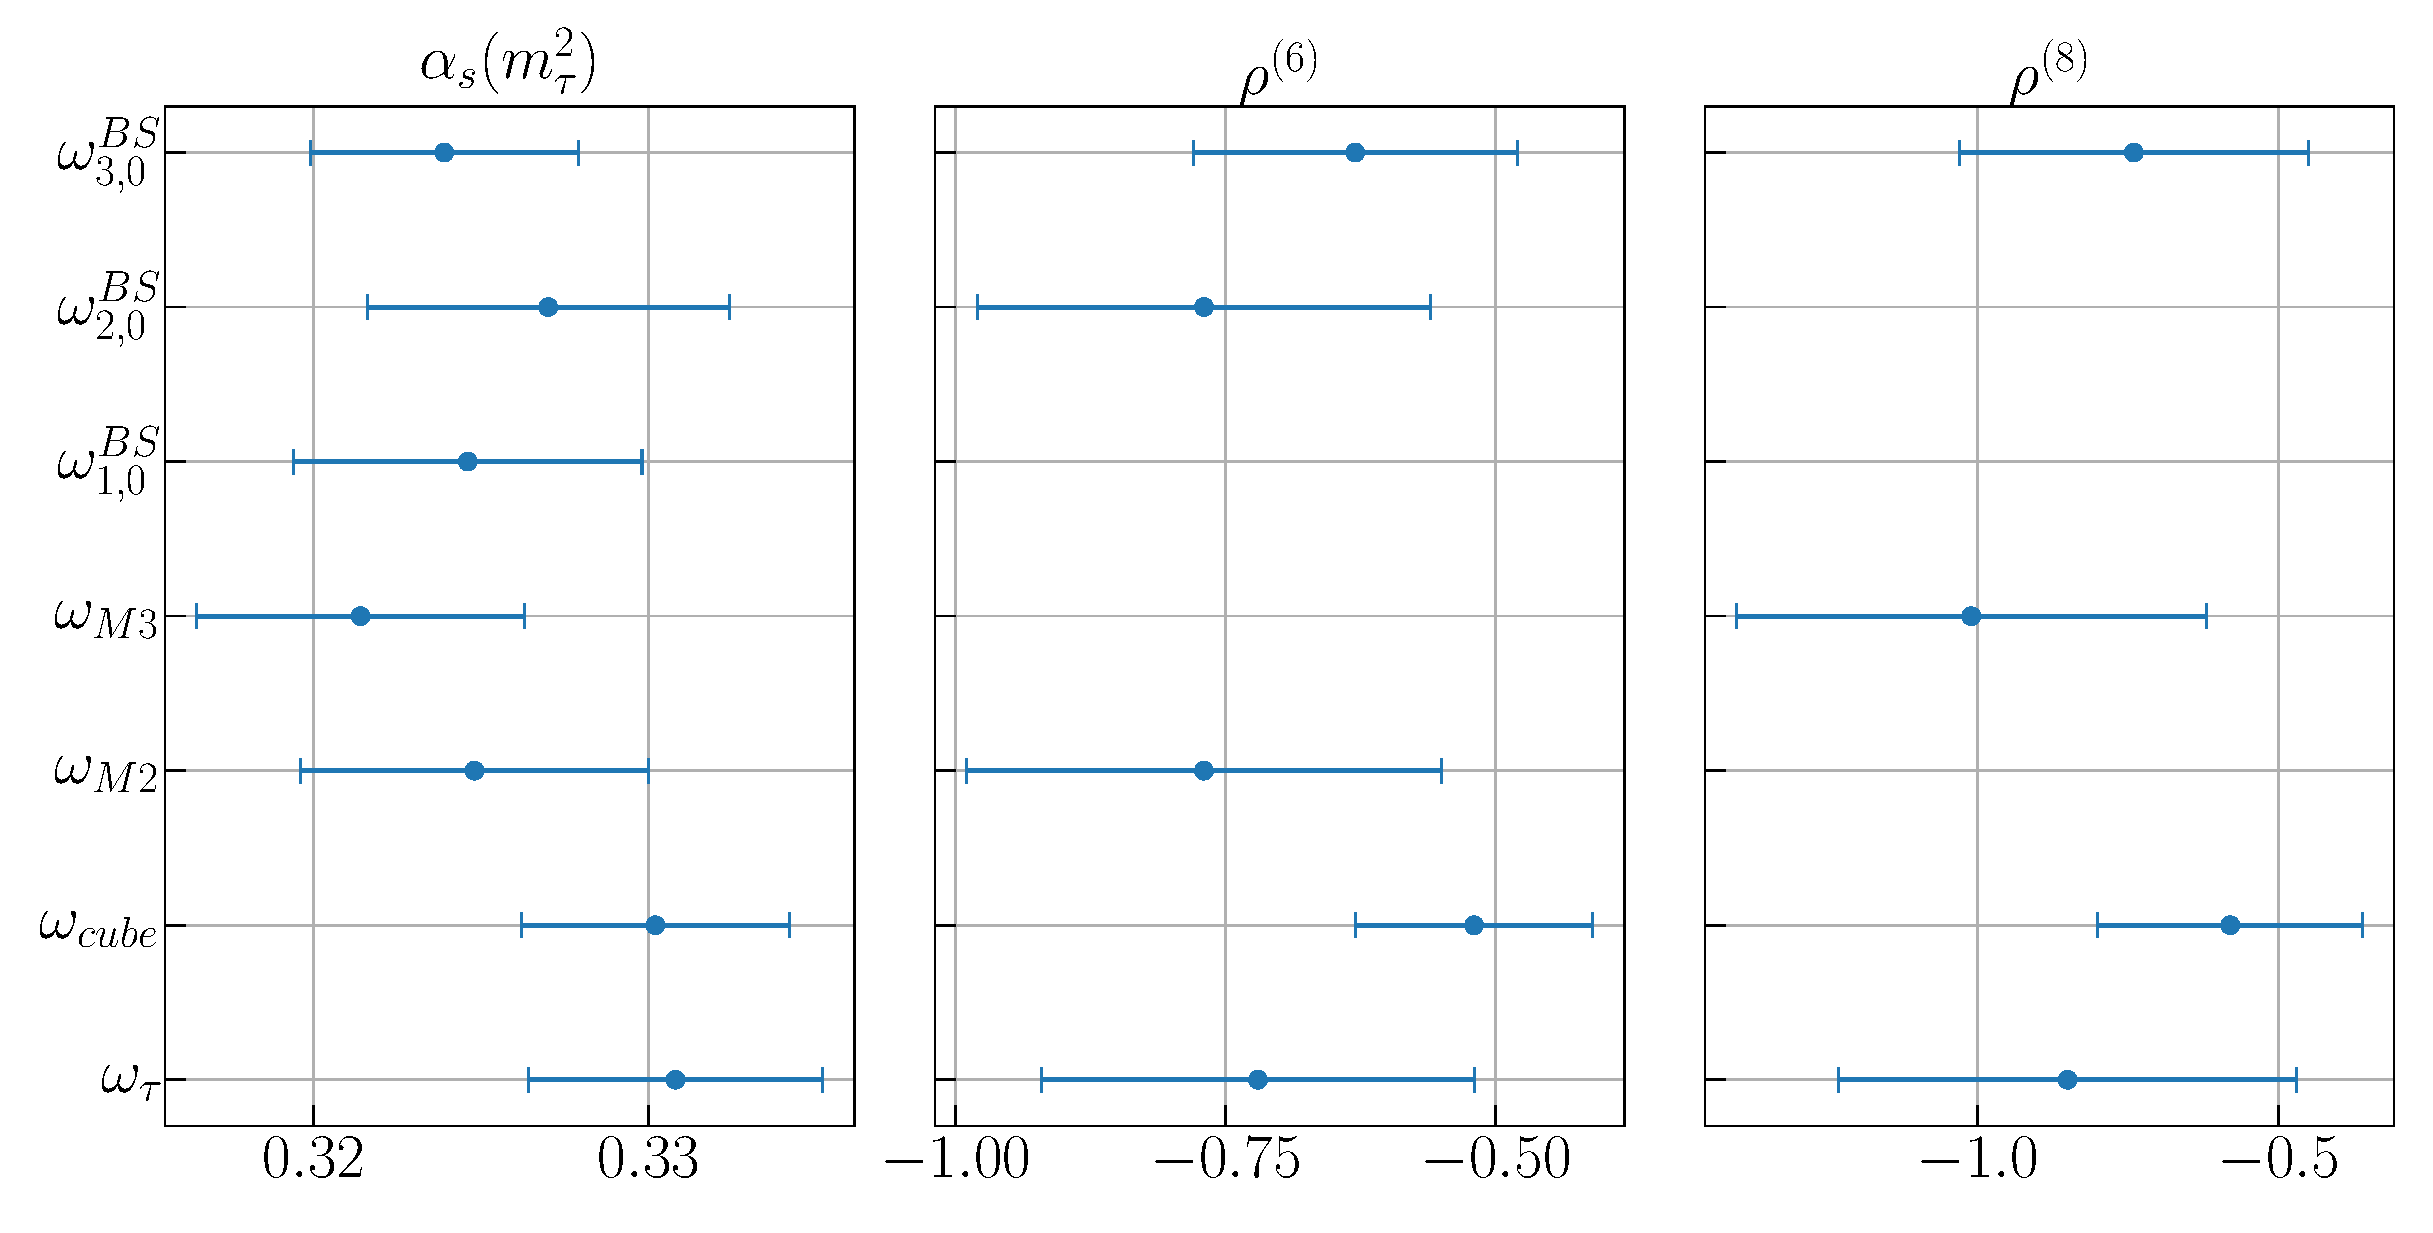
\includegraphics[width=\textwidth]{./images/comparisonAlC6C8.eps}
  \caption{Visual comparison of the fitted parameters \(\alpha_s(m_\tau^2)\),
    \(\rho^{(6)}\) and \(\rho^{(8)}\) for the results of
    \cref{table:fitCombinations}. The values of the different fits and models
    values are very comparable to each other. For the weights including a
    monomial term in \(x\) display the results obtained from the \textsc{bs} as
    can be seen from the upper index of \(\omega_{n,0}^{BS}\).}
  \label{fig:comparisonAlC6C8}
\end{figure}

The high agreement between all fits shows that no \textsc{dv} have to be taken
into account while implementing fits in the \(V+A\) channel and the
corresponding framework, \textsc{fopt} or \textsc{bs} depending if the weight
does not or does include a monomial term in \(x\), for at least single pinched
weights. At least single and not double pinched, because the weights
\(\omega_{M2}\) and \(\omega_{M3}\) are only single pinched, but still in high
agreement with the other higher pinched weights! We consequently do not see any
need to include \textsc{dv} terms in an analysis of \(\alpha_s\) from \(\tau\)
decay data.


\section{Final Results}
Here we will state our final results for the strong coupling and the dimensions
six and eight \textsc{ope} contributions. We have decided to average over all
values of the selected fits seen in \cref{table:fitCombinations}, but focus on
the error given by the \textsc{fopt} fit of the kinematic weight. We did not
want to use the value for the strong coupling of the kinematic weight solely,
because it is representing a rather large value in comparison to the other
selected fits. We further did not want to average over the errors of all
compared fits, as we do not know their correlations. Averaging over all errors
would most probably lead to an underestimated error.

\subsection{Theoretical Error}
The values have a statistical error given by the fitting routine \textsc{minuit}
and a theoretical error. The main contribution from the theoretical error comes
from the fifth Adler function coefficient \(c_{5,1}\), which has not been
calculated yet. Though estimated in \cite{Beneke2008} with a value of \(c_{5,1}
= 283\) we will assume a relative error of \(100\%\) to its value. Consequently,
we performed two additional fits with \(c_{5,1} = 0 \) and \(c_{5,1} = 566\) and
via comparison extracted the error to the central value of the corresponding
parameter. We have further decided instead of stating the resulting asymmetric
errors the larger value of the upper and lower error as a symmetric error. The
results of the additional fits with varying the fifth Adler function coefficient
can be seen in \cref{table:theoreticalError}.
\begin{table}
  \centering
  \begin{tabular}{lcccc}
    \toprule
    & \(c_{5,1} = 0\) & \cellcolor{primary}\(c_{5,1}=283\) & \(c_{5,1}=566\) & \(\Delta\)\\
    \midrule
    \(\alpha_s(m_\tau^2)\) & \(0.3333\) & \cellcolor{primary}\(0.3308\) & \(0.3285\) & \(0.0025\) \\
    \(\rho^{(6)}\) &  \(-0.74\) & \cellcolor{primary}\(-0.72\) & \(-0.69\) & \(0.03\) \\
    \(\rho^{(8)}\) & \(-0.87\) & \cellcolor{primary}\(-0.85\) & \(0.82\) & \(0.03\) \\
    \bottomrule
  \end{tabular}
  \caption{Values of \(\alpha_s, \rho^{(6)}\) and \(\rho^{(8)}\) for varying
    \(c_{5,1}\) and the corresponding, symmetric error \(\Delta\) for each
    parameter to the central value of \(c_{5,1} = 283\).}
  \label{table:theoreticalError}
\end{table}
The symmetrical theoretical errors are then given by \(0.0025, 0.03\) and
\(0.03\) for \(\alpha_s, \rho^{(6)}\) and \(\rho^{(8)}\) correspondingly.

\subsection{Parameter Values}
We will average over the values of \cref{table:fitCombinations} leading to
\begin{tcolorbox}[ams equation,myformula]
  \alpha_s(m_\tau^2) = 0.3261 \pm (0.0044)_{MINUIT} \pm (0.0025)_{c_{5,1}} =
  0.3261 \pm 0.0051
\end{tcolorbox}
for the strong coupling at the \(\tau^2\) scale. The dimension six and eight
\textsc{ope} contributions are very stable in the fits we compared. Consequently
we will state their averaged numerical values
\begin{align}
  \rho^{(6)} &= -0.68 \pm (0.2)_{MINUIT} \pm (0.03)_{c_{5,1}} = -0.68 \pm 0.20\\
  \rho^{(8)} &= -0.80 \pm (0.38)_{MINUIT} \pm (0.03)_{c_{5,1}} = -0.80 \pm 0.38.
\end{align}
Note that the \(\rho^{(6)}\) values from the cubic weight are slightly
different. This is due to the fact, that the cubic weight includes a fourth
fitting parameter, which contribution needs to be compensated by the other
parameters.

The value of higher dimension \textsc{ope} parameters are still compatible but
have a higher variation than the previous two parameters. Beginning from the
\(D=10\) contributions we do not have enough good fits to evaluate their
contribution. Consequently, we do not state a single value for \textsc{ope}
parameters of dimension eight and higher.

\end{document}
% LocalWords:  lllll AlD llll historicAlphasComparison fitCategories ccccc ams
% LocalWords:  kinematicWeight fitWKinAlD cccYYYY fitWCubicAlD fitWCubeAlpha
% LocalWords:  ccYYYYY fitWM ccYYY cubicWeight quarticWeight fitOpt ccYYYY
% LocalWords:  cccccccc ccccccccc fitCombinations comparisonAlC lcccc myformula
% LocalWords:  theoreticalError LocalWords
